\documentclass[11pt,a4paper]{article}

\usepackage[margin=2.3cm]{geometry}
\usepackage{graphicx}
\usepackage{booktabs}
\usepackage{tabularx}
\usepackage{array}
\usepackage{float}
\usepackage{caption}
\usepackage{amsmath}
\usepackage{enumitem}
\usepackage{xcolor}
\usepackage{listings}
\usepackage{fancyhdr}
\usepackage{hyperref}
\usepackage{amsmath}
\usepackage{amssymb}
\hypersetup{colorlinks=true,linkcolor=blue!50!black,urlcolor=blue!50!black}

% ---- code listings ----
\definecolor{codebg}{gray}{0.96}
\definecolor{codekw}{RGB}{0,70,150}
\definecolor{codecm}{RGB}{90,120,90}
\definecolor{codestr}{RGB}{160,60,30}
\lstset{
  language=Python,
  basicstyle=\ttfamily\small,
  keywordstyle=\color{codekw}\bfseries,
  commentstyle=\color{codecm}\itshape,
  stringstyle=\color{codestr},
  backgroundcolor=\color{codebg},
  frame=single, rulecolor=\color{gray!40},
  breaklines=true, columns=fullflexible,
  showstringspaces=false, aboveskip=8pt, belowskip=8pt
}

\newcommand{\col}[1]{\texttt{#1}}
% Red marker for values that still have to be filled in by hand.
\newcommand{\fillin}[1]{\textcolor{red}{\textbf{[#1]}}}
\setlist{itemsep=2pt,topsep=4pt}
\setlength{\emergencystretch}{2em}
\renewcommand{\arraystretch}{1.18}

\pagestyle{fancy}
\fancyhf{}
\setlength{\headheight}{14pt}
\lhead{Artificial Intelligence -- Homework 2}
\rhead{Omid Basafa}
\cfoot{\thepage}

% =====================================================================
\begin{document}

% ------------------------------ title page ---------------------------
\begin{titlepage}
  \centering
  \vspace*{1cm}
  
\includegraphics[width=0.28\textwidth]{iust-logo.png}\par
  \vspace{0.8cm}
  {\Large Iran University of Science and Technology\par}
  \vspace{0.3cm}
  {\large School of Computer Engineering\par}
  \vspace{1.6cm}
  {\Huge\bfseries Artificial Intelligence\par}
  \vspace{0.6cm}
  {\LARGE Homework 2: Commute Optimizer\par}
  \vspace{0.3cm}
  {\large Local search for urban trip planning\par}
  \vfill
  \begin{tabular}{rl}
    \textbf{Student name:}   & Omid Basafa \\[4pt]
    \textbf{Student number:} & 403521078 \\
  \end{tabular}
  \vfill
  {\large \today\par}
\end{titlepage}

\tableofcontents
\newpage

% =====================================================================
\section{Implementation Logic}

A state is a pair $x = \langle P, t_{\text{start}} \rangle$. The cost $f(x)$ is the travel
time from the FIFO simulator in \col{core/problem.py}. All four solvers use the same operators
from \col{algorithms/operators.py}, so the differences between them come only from how they choose
among the moves. The code below is taken from the project with docstrings and type hints removed,
and for the solvers only the main part of \col{solve} is shown.

\subsection{Time moves}

A time move keeps the path and shifts the departure by one step of $\pm\Delta t$.

\begin{lstlisting}
def snap_time(t, problem):
    t = min(max(t, problem.t_min), problem.t_max)
    k = round((t - problem.t_min) / problem.t_step)
    # Largest k that still lies inside the window (handles t_max not on the grid).
    k_max = int((problem.t_max - problem.t_min) / problem.t_step + 1e-9)
    k = min(max(k, 0), k_max)
    return round(problem.t_min + k * problem.t_step, 2)

def time_moves(s, problem):
    out = []
    t_start = s.departure_time
    for k in (-1, 1):
        t = snap_time(t_start + k * problem.t_step, problem)
        if t != t_start:
            out.append(State(s.path, t))
    return out
\end{lstlisting}

\noindent \col{snap\_time} does two jobs: it clamps a time into $[t_{\min}, t_{\max}]$ and rounds it
to the nearest point of the grid $t_{\min} + k\Delta t$. Time moves and crossover both use it, so
neither can produce an off-grid time. At the edge of the window the clamp returns the
same time, and the check \col{t != t\_start} drops that move. For example, at 07:00 only the
move to 07:05 is generated.

\subsection{Route moves}

A route move keeps the departure time and replaces one stretch of the path with a different detour.
The detours come from a depth-first search:

\begin{lstlisting}
def simple_paths(problem, src, dst, forbidden, max_edges):
    out = []
    stack = [(src, (src,))]
    while stack:
        node, sofar = stack.pop()
        if node == dst:
            out.append(sofar)
            continue
        if len(sofar) - 1 >= max_edges:
            continue
        for nxt in problem.network.get_neighbors(node):
            if nxt not in forbidden and nxt not in sofar:
                stack.append((nxt, sofar + (nxt,)))
    return out
\end{lstlisting}

\noindent Each stack entry holds the current node and the path walked so far. A branch ends when it
reaches \col{dst} or uses up \col{max\_edges}. Because it only follows \col{get\_neighbors}, every
edge in a detour is a real road. \col{route\_moves} calls this search for every stretch of the path:

\begin{lstlisting}
MAX_SPAN = 4      # longest stretch of the path one move may replace
MAX_DETOUR = 5    # longest detour one move may insert

def route_moves(s, problem):
    p, out = s.path, []
    for i in range(len(p) - 1):
        for j in range(i + 1, min(len(p), i + MAX_SPAN + 1)):
            # Detour must not reuse any node kept from the rest of the path.
            forbidden = set(p[:i]) | set(p[j + 1:])
            for seg in simple_paths(problem, p[i], p[j], forbidden, MAX_DETOUR):
                if seg != p[i : j + 1]:
                    out.append(State(p[:i] + seg + p[j + 1:], s.departure_time))
    return out
\end{lstlisting}

\noindent\textbf{Example.} On \col{metropolis\_graph}, take the path Home, C1, C2, C3, C4, Uni with
$i = 2$ (C2) and $j = 5$ (Uni). The kept nodes are Home and C1, so these are forbidden. The search
finds detours such as C2, B2, Uni, which gives the new path Home, C1, C2, B2, Uni. C3 and C4 are not
forbidden, because the old stretch is being removed and a detour may use them again.

\subsection{Combining the moves}

\begin{lstlisting}
def get_neighbors(state, problem):
    seen, out = {state}, []
    for n in time_moves(state, problem) + route_moves(state, problem):
        if n not in seen and problem.is_valid_state(n):
            seen.add(n)
            out.append(n)
    return out
\end{lstlisting}

\noindent Each move changes either the time or the path, never both. \col{seen} starts with the
current state, so a state is never its own neighbor, and two different moves that give the same path
count once. Only 2 neighbors are time moves and the rest are route moves. The neighborhood is around
16 states on \col{metropolis\_graph} and grows quickly on denser maps. This has a direct effect on SA,
which picks uniformly from the list and so rarely picks a time move.

\subsection{How paths stay loop-free}

Loops are prevented when a move is built, and then checked again:

\begin{enumerate}
  \item \textbf{Forbidden set.} When replacing $p_i \dots p_j$, the nodes that stay in the path
  ($p_0 \dots p_{i-1}$ and $p_{j+1} \dots p_m$) are forbidden for the detour.
  \item \textbf{DFS check.} The DFS only moves to a node that is neither forbidden nor already on
  the current detour (\col{nxt not in sofar}). So the detour has no loop inside it and cannot touch
  the kept parts.
  \item \textbf{Splice.} The new path is \col{p[:i] + seg + p[j+1:]}. These three parts share no
  nodes, so the result is simple by construction. \col{seg} starts at $p_i$ and ends at $p_j$, which
  are exactly the points where the kept parts need to connect, so the path also stays connected.
  \item \textbf{Final filter.} \col{get\_neighbors} still calls \col{is\_valid\_state} on every
  candidate. This is only a safety net, since a candidate should never fail here.
\end{enumerate}

\paragraph{Are paths left unexplored?}
Inside its limits the neighborhood is exhaustive: all waypoint pairs are tried and the DFS lists
every valid detour, so no local alternative is skipped. Going further takes several moves in a
row. Random restarts, the random initial populations and crossover are what reach routes far from
the current one. This is not a guarantee that every path gets visited, because that would be brute
force (see Question 7).

\subsection{Random states}

Restarts and initial populations need valid states from anywhere in the space:

\begin{lstlisting}
def random_path(problem, rng):
    dst = problem.destination
    first = list(problem.network.get_neighbors(problem.origin))
    rng.shuffle(first)
    stack = [(problem.origin, iter(first))]
    on_path = {problem.origin}
    while stack:
        node, untried = stack[-1]
        if node == dst:
            return tuple(n for n, _ in stack)
        nxt = next((v for v in untried if v not in on_path), None)
        if nxt is None:
            stack.pop()
            on_path.discard(node)
            continue
        succ = list(problem.network.get_neighbors(nxt))
        rng.shuffle(succ)
        stack.append((nxt, iter(succ)))
        on_path.add(nxt)
    return None
\end{lstlisting}

\noindent This is a randomized DFS with backtracking. The stack is the path itself, and \col{on\_path}
stops it from revisiting a node, so the result is loop-free too. At a dead end it steps back and tries
another branch, so it finds a path whenever one exists. \col{random\_state} then adds a random time
from the valid domain. The paths can be long and winding because the search stops at the first arrival
at Uni, which is fine: their job is to give diversity, and the search then improves them.

\subsection{Crossover}

\begin{lstlisting}
def blend_time(t1, t2, problem):
    lo, hi = min(t1, t2), max(t1, t2)
    return snap_time(random.uniform(lo, hi), problem)

def crossover(parent1, parent2, problem):
    p1, p2 = parent1.path, parent2.path
    t = blend_time(parent1.departure_time, parent2.departure_time, problem)

    # Shared intermediate junctions (origin/destination are trivially shared).
    pos2 = {node: k for k, node in enumerate(p2)}
    candidates = []
    for i in range(1, len(p1) - 1):
        j = pos2.get(p1[i])
        if j is None or j in (0, len(p2) - 1):
            continue
        # Both splice directions at this pivot: head of one + tail of the other.
        for child in (p1[:i] + p2[j:], p2[:j] + p1[i:]):
            if child not in (p1, p2) and len(child) == len(set(child)):
                candidates.append(child)

    if candidates:
        child = State(random.choice(candidates), t)
        if problem.is_valid_state(child):
            return child

    # Fallback: parents share no usable junction -> mutate one parent.
    base = State(random.choice((p1, p2)), t)
    neighbors = get_neighbors(base, problem)
    return random.choice(neighbors) if neighbors else base
\end{lstlisting}

\noindent\textbf{Path.} \col{pos2} gives the position of each node of $P_2$, so shared nodes are found
in one pass over $P_1$. Each shared node gives two children. For example, with parents Home, N1, B1,
C2, C3, C4, Uni and Home, S1, T1, C2, B2, Uni, the pivot C2 gives:
\begin{itemize}
  \item Home, N1, B1, C2, B2, Uni
  \item Home, S1, T1, C2, C3, C4, Uni
\end{itemize}
The edges are always valid, since each one comes from a parent and the two parts join at the shared
node. A loop is still possible when the head of one parent contains a node from the tail of the other,
so \col{len(child) == len(set(child))} rejects those children. Copies of a parent are rejected too.

\noindent\textbf{Time.} The child's time is a random point between the parents' times, snapped to the
grid. On average this equals their mean, and the randomness gives more variety than an exact midpoint.

\noindent\textbf{Fallback.} If no pivot works, the child is a random neighbor of one parent with the
blended time. So crossover always returns a valid state, even for completely disjoint parents.

\subsection{Tracking the best state}

All solvers record their progress the same way, through a small \col{Tracker} class in
\col{algorithms/base.py}:

\begin{lstlisting}
def offer(self, s, c):
    if c < self.best_cost - EPS:
        self.best, self.best_cost, self.found_at = s, c, len(self.history)

def tick(self):
    self.history.append(self.best_cost)
\end{lstlisting}

\noindent \col{offer} keeps the best state ever seen and \col{tick} closes a step by saving the best
cost so far. So a solver can move to a worse state without losing its best answer, and this is also
why the convergence curves can never go up.

\subsection{Hill Climbing}

\begin{lstlisting}
for restart in range(self.max_restarts + 1):
    cur = (
        self.problem.generate_initial_state()
        if restart == 0
        else random_state(self.problem, self.rng)
    )
    cur_cost = f(cur)
    tr.offer(cur, cur_cost)
    tr.tick()

    sideways_left = self.max_sideways
    tabu = {cur}  # states visited in this climb (prevents plateau ping-pong)
    for _ in range(self.max_steps):
        cand = [n for n in get_neighbors(cur, self.problem) if n not in tabu]
        if not cand:
            break

        costs = [f(n) for n in cand]
        best_c = min(costs)
        nxt_states = [n for n, c in zip(cand, costs) if c <= best_c + EPS]
        nxt = self.rng.choice(seq=nxt_states)
        if best_c + EPS < cur_cost:
            cur, cur_cost = nxt, best_c
        elif abs(best_c - cur_cost) <= EPS and sideways_left > 0:
            cur, cur_cost = nxt, best_c
            sideways_left -= 1
        else:
            break

        tabu.add(cur)
        tr.offer(cur, cur_cost)
        tr.tick()
\end{lstlisting}

\noindent This is steepest descent: every step evaluates all neighbors and takes the best one, with
ties broken randomly. There are three cases:
\begin{itemize}
  \item \textbf{Better neighbor:} move to it.
  \item \textbf{Equal neighbor:} move to it if the sideways budget is not used up. The budget
  (\col{max\_sideways} = 100) is set once per climb and is not refilled after an improvement.
  \item \textbf{Only worse neighbors:} the climb has reached a local minimum and it ends.
\end{itemize}
Without the \col{tabu} set, a sideways move could go from A to B and straight back to A until the
budget ran out. Excluding visited states forces the climb to walk across a plateau instead. There are
11 climbs in total: the initial state plus \col{max\_restarts} = 10 restarts from \col{random\_state}.
The budget and \col{tabu} set reset for each climb, while the \col{Tracker} keeps the best result
across all of them. Each climb is also capped at \col{max\_steps}, which is 500 by default.

\subsection{Simulated Annealing}

\begin{lstlisting}
T = self.initial_temp
cur = self.problem.generate_initial_state()
cur_cost = f(cur)
tr.offer(cur, cur_cost)
for _ in range(self.max_iterations):
    if T < self.min_temp:
        break

    neighbors = get_neighbors(cur, self.problem)
    if not neighbors:
        break
    nxt = self.rng.choice(neighbors)
    nxt_cost = f(nxt)

    if nxt_cost < math.inf:
        dE = nxt_cost - cur_cost
        if dE <= 0 or self.rng.random() < math.exp(-dE / T):
            cur, cur_cost = nxt, nxt_cost
            tr.offer(cur, cur_cost)

    T *= self.cooling_rate
    tr.tick()
\end{lstlisting}

\noindent Each iteration evaluates one random neighbor, unlike HC which evaluates all of them. Moves
with $\Delta E \le 0$ are always accepted, and a worse move is accepted with the Metropolis probability
$\exp(-\Delta E / T)$. So a large $T$ accepts almost anything, and a small $T$ behaves like a randomized
hill climb.

The temperature drops by $T_{k+1} = \alpha T_k$ on every iteration, whether or not the move was
accepted. The run therefore lasts about $\ln(T_0 / T_{\min}) / (-\ln \alpha)$ iterations. With
$T_0 = 120$, $\alpha = 0.992$ and $T_{\min} = 0.001$ this is about 1457, so the limit of 3000 is never
reached. Note that the whole neighborhood is built on every iteration just to pick one state from it,
so an SA iteration is not as cheap as it first looks.

\subsection{Local Beam Search}

\begin{lstlisting}
beam = self.distinct_random_states()
for s in beam:
    tr.offer(s, c(s))
tr.tick()

for _ in range(self.max_iterations):
    # dict, not set: keeps insertion order, so ties rank the same on every run.
    pool = dict.fromkeys(beam)
    for s in beam:
        pool.update(dict.fromkeys(get_neighbors(s, self.problem)))
    ranked = sorted(pool, key=c)

    # Diversity: first take the best state of each *distinct path*, and only
    # then fill remaining slots with same-path/different-time variants.
    new_beam, seen_paths, rest = [], set(), []
    for s in ranked:
        if s.path not in seen_paths and len(new_beam) < self.beam_width:
            new_beam.append(s)
            seen_paths.add(s.path)
        else:
            rest.append(s)
    new_beam += rest[: self.beam_width - len(new_beam)]
    new_beam.sort(key=c)

    for s in new_beam:
        tr.offer(s, c(s))
    tr.tick()

    if set(new_beam) == set(beam):  # beam stopped changing -> converged
        break
    beam = new_beam
\end{lstlisting}

\noindent The beam starts with $K = 8$ distinct states: the initial state plus 7 random ones. The main
point is that all successors go into one shared pool. This is what separates beam search from 8
independent climbs: if one state has many good neighbors, they can take most of the slots and the weak
states are dropped. The current beam is also in the pool, so the best cost never gets worse.

A plain ``top 8'' would collapse quickly, because one good route at 8 neighboring departure times
would fill the whole beam. So the selection walks through the ranked list and first takes the best state of each
distinct path. Skipped states go to \col{rest}, in rank order, and only fill the slots that remain if
there are too few distinct paths. The search stops when the beam stays the same for a full step. The
memoized cost function \col{c} evaluates each state only once, because neighborhoods overlap heavily.

\subsection{Genetic Algorithm}

\begin{lstlisting}
def pick_parent(self, pop, costs, size):
    return min(self.rng.sample(pop, k=min(size, len(pop))), key=costs.__getitem__)

# inside solve():
costs = {}
for _ in range(self.generations):
    for s in pop:
        if s not in costs:
            costs[s] = f(s)
    for s in pop:
        tr.offer(s, costs[s])
    ranked = sorted(pop, key=costs.__getitem__)
    nxt = ranked[: self.elitism]
    while len(nxt) < self.population_size:
        p1 = self.pick_parent(pop, costs, self.tournament_size)
        p2 = self.pick_parent(pop, costs, self.tournament_size)
        child = (
            crossover(p1, p2, self.problem)
            if self.rng.random() < self.crossover_rate
            else p1
        )

        if self.rng.random() < self.mutation_rate:
            neighs = get_neighbors(child, self.problem)
            if neighs:
                child = self.rng.choice(neighs)
        nxt.append(child)
    pop = nxt
    tr.tick()
\end{lstlisting}

\noindent The settings are population 50 and 120 generations. Each generation has these parts:
\begin{itemize}
  \item \textbf{Fitness.} Lower $f(x)$ means higher fitness, so the cost is used directly. Costs are
  cached in a dictionary because good individuals survive across generations.
  \item \textbf{Selection.} Tournament of size 3: take 3 random individuals and keep the best. Weak
  individuals can still win if the other two picked are also weak, which keeps some diversity. A
  larger tournament would increase the selection pressure.
  \item \textbf{Crossover.} With rate 0.85 the child comes from \col{crossover}; otherwise it is a copy
  of the first parent.
  \item \textbf{Mutation.} With rate 0.25 the child is replaced by a random neighbor, so mutation is
  one move of the same kind the other algorithms use.
  \item \textbf{Elitism.} The best 3 individuals are copied directly without change, so the best
  solution in the population can never be lost.
\end{itemize}

% =====================================================================
\section{Performance Comparison}

\subsection{Main comparison: megacity}

Table~\ref{tab:main} compares the algorithms on the \col{megacity} map (168 nodes) with the
\col{megacity\_rush} scenario. Best cost, departure and runtime come from a run with seed 42. The
program does not print step counts, so these are read from the plot in Figure~\ref{fig:conv}, which
is a separate run. Both runs are shown side by side so their values are not mixed. Marked step counts
are approximate, and the second number is the total length of the run.

\begin{table}[H]
\centering
\caption{The four algorithms on \col{megacity / megacity\_rush}.}
\label{tab:main}
\small
\setlength{\tabcolsep}{5pt}
\begin{tabular}{lccccc}
\toprule
 & \multicolumn{3}{c}{\textbf{Seed 42 run}} & \multicolumn{2}{c}{\textbf{Run in Figure~\ref{fig:conv}}} \\
\cmidrule(lr){2-4}\cmidrule(lr){5-6}
\textbf{Algorithm} & \textbf{$f(x^*)$ (min)} & \textbf{Departure} & \textbf{Runtime (s)} & \textbf{$f(x^*)$ (min)} & \textbf{Steps (conv. / total)} \\
\midrule
Hill Climbing       & 89.50 & 10:00 & 1.223 & 89.00 & $\approx$26 / $\approx$127 \\
Simulated Annealing & 136.31 & 07:00 & 4.896 & 94.56 & $\approx$740 / $\approx$1457 \\
Local Beam Search   & 91.20 & 10:00 & 0.795 & 91.20 & 11 / 14 \\
Genetic Algorithm   & \textbf{88.60} & 10:00 & 10.338 & \textbf{88.60} & $\approx$12 / 121 \\
\bottomrule
\end{tabular}
\end{table}


\noindent What the seed 42 run shows:
\begin{itemize}
  \item \textbf{GA} has the best cost and the longest runtime. Its route has a free-flow time of 88.60
  minutes, the shortest on the map, and congestion can only add to that. So its result is within 0.002
  minutes of the best possible.
  \item \textbf{HC} is the best trade-off: only 0.90 minutes behind GA in about one eighth of the time.
  \item \textbf{Beam} is the fastest, but 2.60 minutes behind GA.
  \item \textbf{SA} returned its starting state (the shortest route at 07:00), so in this run it never
  found anything better. It uses the same route as GA, and the whole 47.71-minute difference comes
  from the departure time.
\end{itemize}
HC, Beam and GA all chose 10:00, when traffic has almost cleared: each cost is within 0.003 minutes of
that route's free-flow time. At that hour, the only thing separating them is the quality of the route.

\noindent The step counts are not equal units of work. One HC step scans a whole neighborhood, one SA
step evaluates a single neighbor, one beam step expands 8 neighborhoods, and one GA step makes a
whole generation. Runtime is the fairer measure of cost.

\subsection{Runs with the rush\_hour scenario}

\begin{table}[H]
\centering
\caption{Seed 42 runs using the \col{rush\_hour} scenario on larger maps.}
\label{tab:rush}
\small
\setlength{\tabcolsep}{5pt}
\begin{tabular}{lcccccc}
\toprule
 & \multicolumn{3}{c}{\textbf{metropolis\_graph (16 nodes)}} & \multicolumn{3}{c}{\textbf{megacity (168 nodes)}} \\
\cmidrule(lr){2-4}\cmidrule(lr){5-7}
\textbf{Algorithm} & \textbf{$f(x^*)$} & \textbf{Departure} & \textbf{Runtime (s)} & \textbf{$f(x^*)$} & \textbf{Departure} & \textbf{Runtime (s)} \\
\midrule
Hill Climbing       & 31.00 & 07:00 & 0.063 & 88.60 & 07:00 & 0.836 \\
Simulated Annealing & 31.00 & 07:00 & 0.313 & 88.60 & 07:00 & 5.357 \\
Local Beam Search   & 31.00 & 07:00 & 0.005 & 88.60 & 07:00 & 0.067 \\
Genetic Algorithm   & 31.00 & 07:00 & 1.254 & 88.60 & 07:00 & 11.976 \\
\bottomrule
\end{tabular}
\end{table}

\noindent All algorithms return the same result here, but this says nothing about search quality.
The peaks in \col{rush\_hour} are defined on \col{toy\_graph} edges (such as Home to H1), and none of
those edges exist on these two maps, so there is no traffic at all. The cost is then the same at every
departure time, and the initial state is already the free-flow shortest route. Nothing can improve on
it, and it stays at 07:00 because only a strictly better state replaces the best one. Only the runtimes
are useful in this table. The route is Home, C1, C2, B2, Uni on \col{metropolis\_graph}, and the GA
route of Table~\ref{tab:routes} on \col{megacity}.

\subsection{All scenarios}

Table~\ref{tab:all} uses the values from the convergence figures, so its \col{megacity} row matches the
right-hand side of Table~\ref{tab:main}.

\begin{table}[H]
\centering
\caption{Best $f(x^*)$ in minutes for each map with its own scenario (one run each).}
\label{tab:all}
\begin{tabular}{llrrrr}
\toprule
\textbf{Map (nodes)} & \textbf{Scenario} & \textbf{HC} & \textbf{SA} & \textbf{Beam} & \textbf{GA} \\
\midrule
toy\_graph (7)         & rush\_hour            & 30.00 & 30.00 & 30.00 & 30.00 \\
downtown\_grid (12)    & flat\_plateau         & 25.07 & 25.07 & 25.07 & 25.07 \\
metropolis\_graph (16) & cascading\_gridlock   & 31.00 & 31.10 & 31.00 & 31.00 \\
metropolis\_graph (16) & crossover\_showcase   & 31.00 & 31.00 & 31.00 & 31.00 \\
metropolis\_graph (16) & dual\_peak\_rush\_hour & 31.00 & 31.08 & 31.00 & 31.00 \\
big\_city (90)         & big\_city\_rush       & 56.03 & 72.12 & 73.82 & \textbf{55.43} \\
megacity (168)         & megacity\_rush        & 89.00 & 94.56 & 91.20 & \textbf{88.60} \\
\bottomrule
\end{tabular}
\end{table}

% =====================================================================
\section{Convergence and Landscape Analysis}

\begin{figure}[H]
\centering
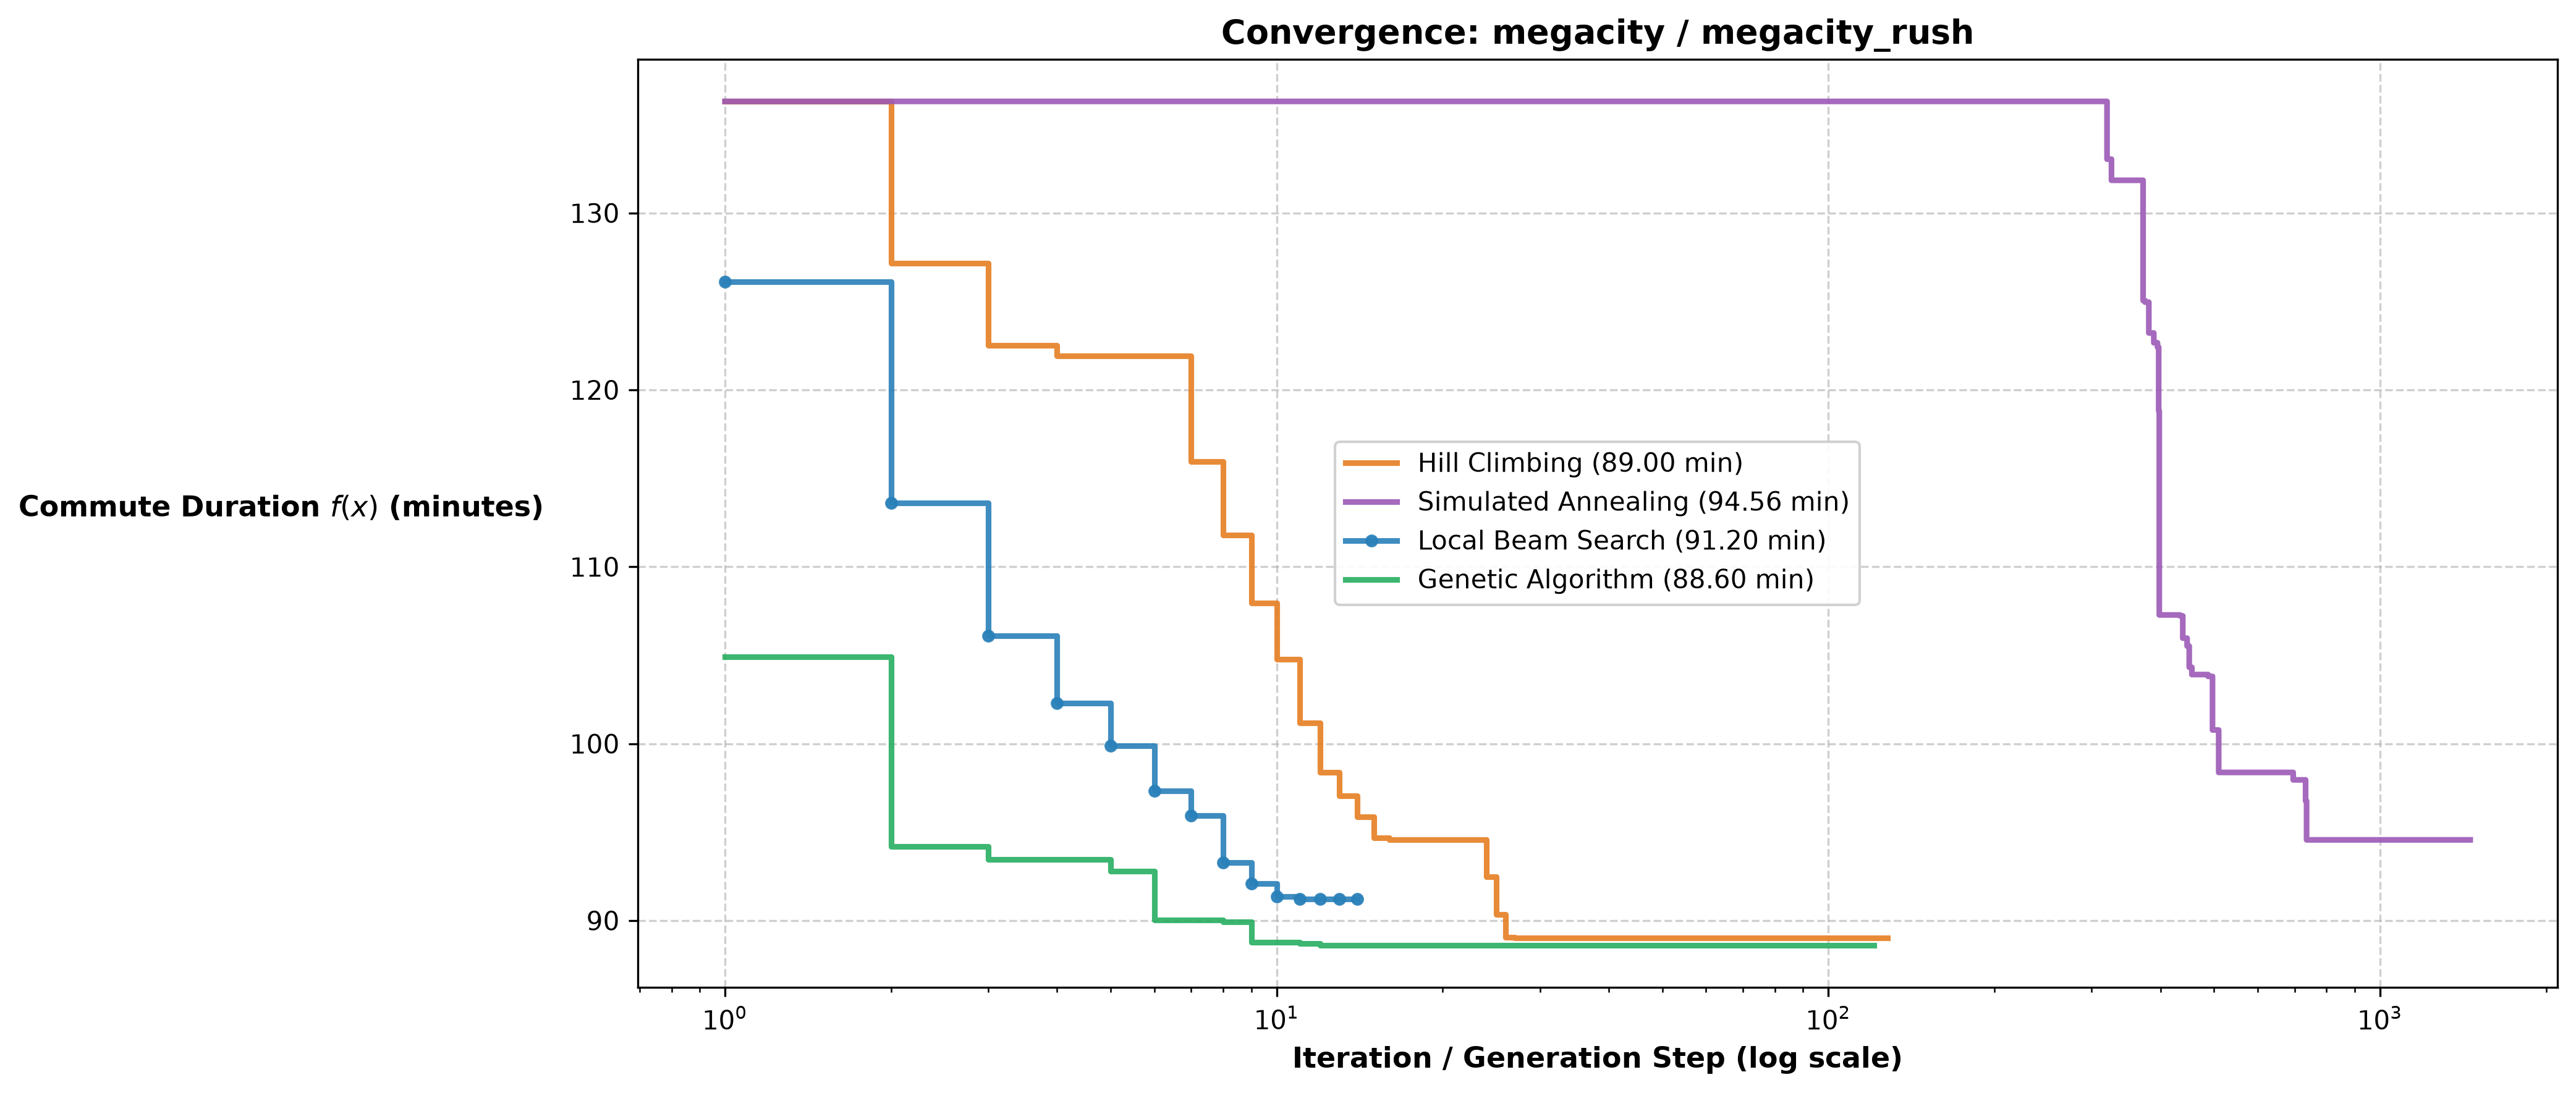
\includegraphics[width=\textwidth]{figures/convergence_comparison.png}
\caption{Convergence on \col{megacity / megacity\_rush}. The curves show the \emph{best cost so
far}, so the worse moves SA accepts do not appear in them.}
\label{fig:conv}
\end{figure}

\begin{figure}[H]
\centering
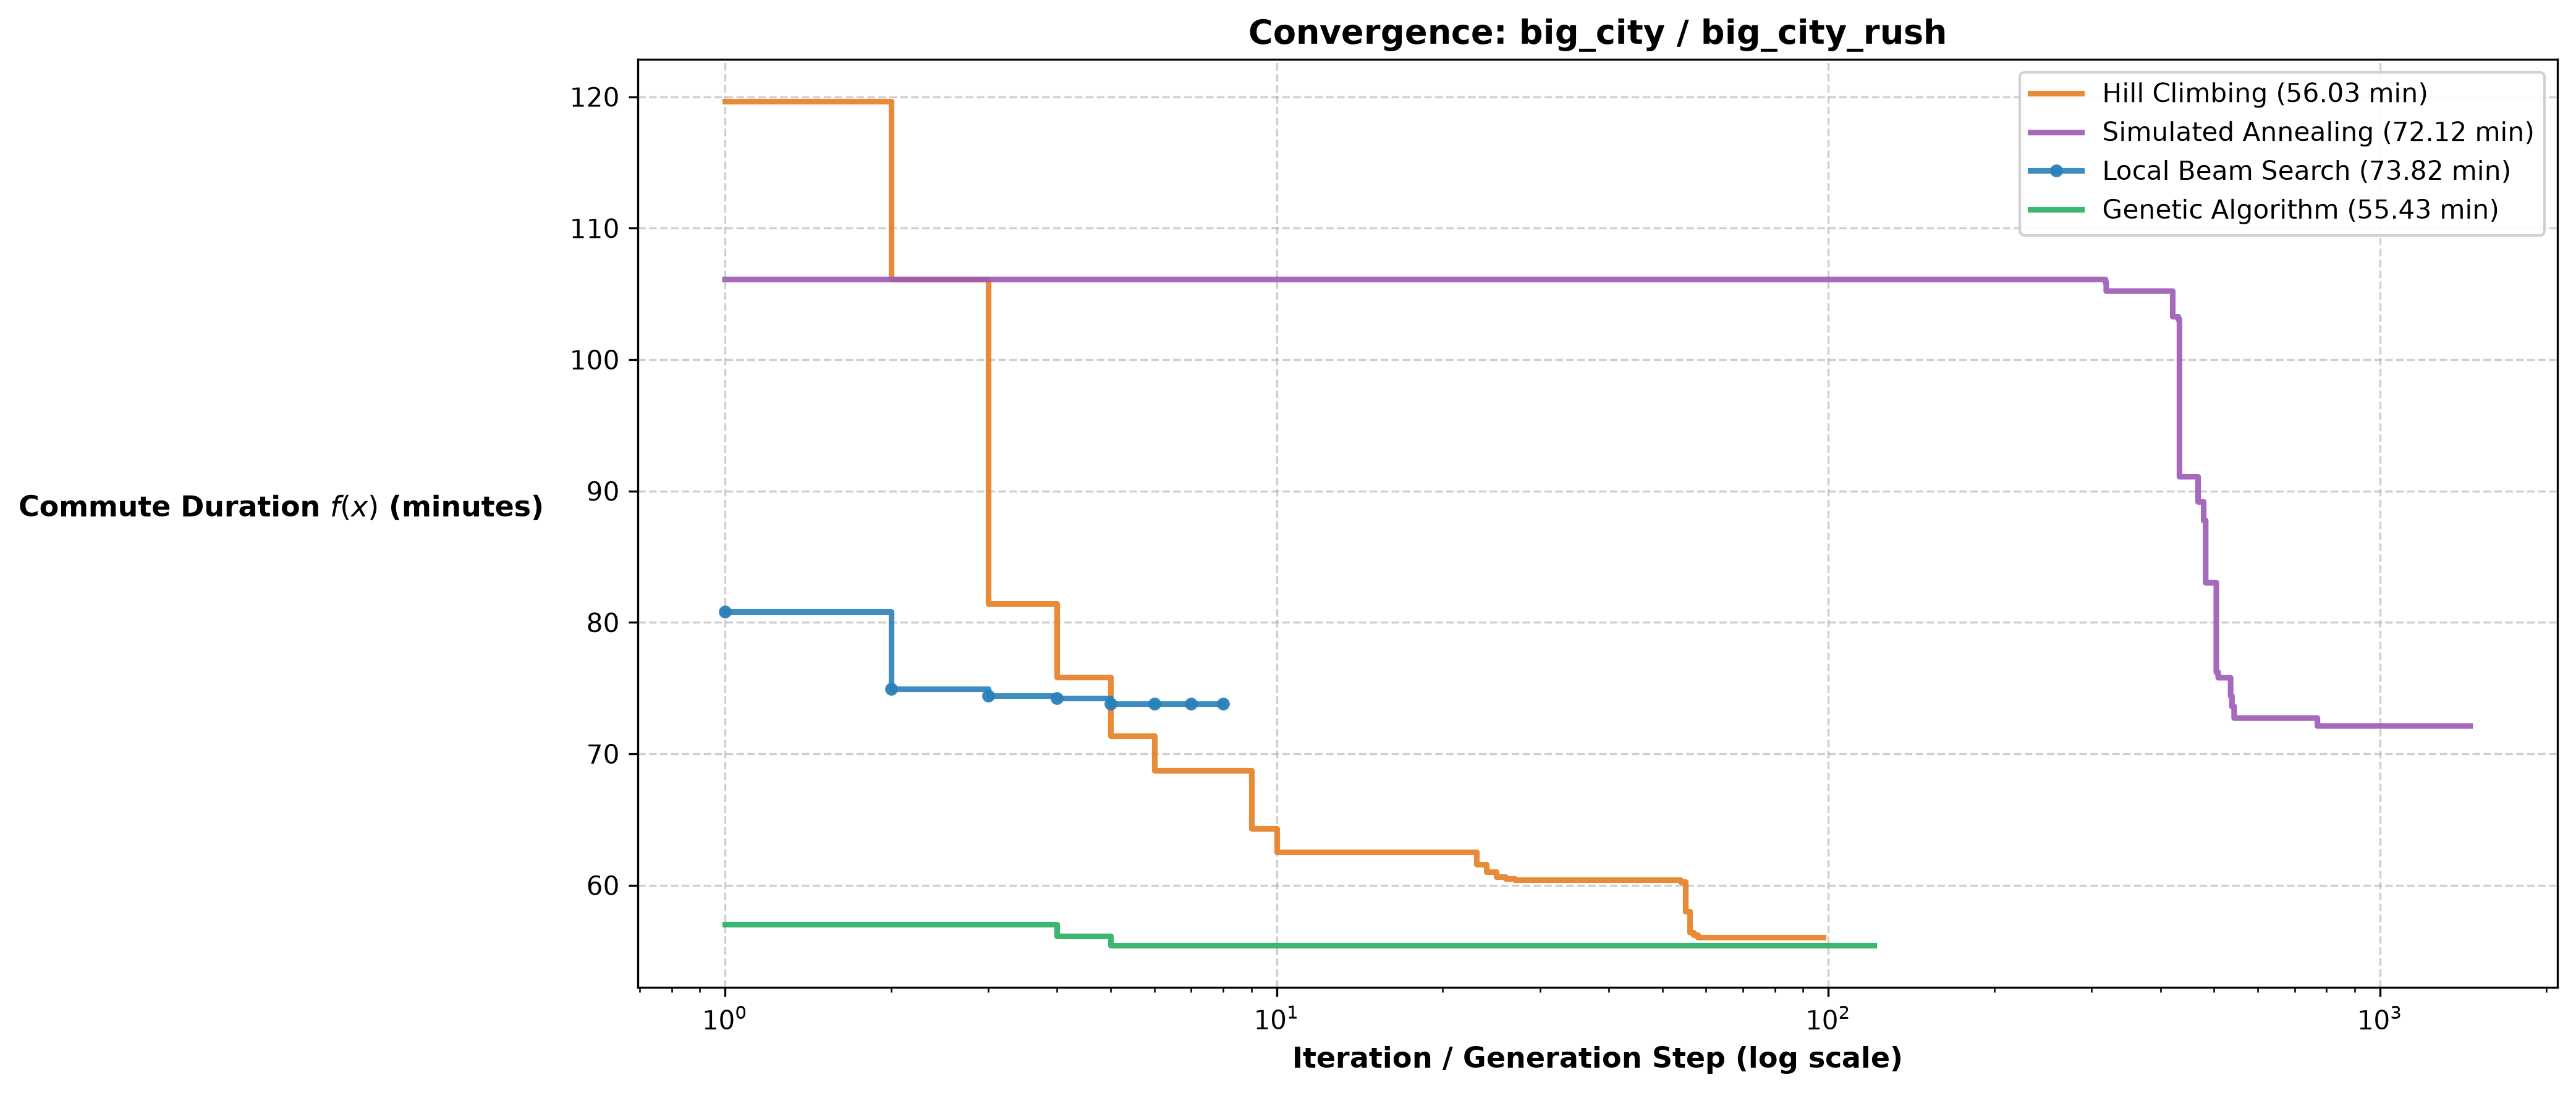
\includegraphics[width=\textwidth]{figures/big_city_rush.png}
\caption{Convergence on \col{big\_city / big\_city\_rush}, where the gap between the algorithms is largest.}
\label{fig:big}
\end{figure}

\paragraph{Small versus large maps.} On the small maps almost everything reaches the same answer,
and these answers are close to free flow. On \col{metropolis\_graph}, 31.00 is exactly the free-flow
shortest route (Home, C1, C2, B2 or T2, Uni). The landscape only becomes hard on the two large maps,
which were built with a ``highway trap'': fast express links that get the heaviest congestion. There
the order is clear: GA and HC are close at the top, while Beam and SA are well behind.

\paragraph{Plateaus.} On \col{flat\_plateau} every algorithm finds 25.07 (Figure~\ref{fig:others}).
Working it out by hand, this is the 25-minute free-flow path Home, G1, G2, G3, G7, Uni leaving at
10:00, plus a small Gaussian tail. HC gets there in about 10 steps, so this plateau did not trap it.
Flat stretches in a best-so-far curve are not always real plateaus, though. HC's long flat parts on
\col{big\_city} (around steps 10--23 and 27--54) are most likely climbs and restarts that did not
beat the best value yet, since that map has few exact ties.

\paragraph{Peaks.} A rush-hour peak is a hill in the time dimension: crossing it takes several
5-minute steps that each make the cost worse. HC cannot do this within one climb and depends on a
restart landing on the other side. SA can cross while it is hot, and GA can jump over it because
random initial times and blending are not limited to one $\Delta t$. The size of this effect is clear
in the seed 42 run on \col{megacity}: the same route costs 136.31 minutes at 07:00 and 88.60 at 10:00.

\paragraph{Valleys and local minima.}
\begin{itemize}
  \item \textbf{GA} was the best on both large maps, and on \col{megacity} it is essentially at the
  free-flow limit (88.60). Its 50 random starts already land in good
  valleys (57.0 on \col{big\_city} in the first generation, better than the final result of SA and
  Beam), and crossover then joins good route sections. It settles very early, around generation 12
  on \col{megacity}, so most of its 120 generations add nothing.
  \item \textbf{HC} is close behind. A single climb stops at the bottom of its valley, but restarts
  sample new ones. On \col{big\_city} the last big gain comes late (around step 58 of 99), which shows
  the restarts are doing real work.
  \item \textbf{Beam} converges fast and then gets stuck: it stopped after 14 steps on \col{megacity}
  and 8 on \col{big\_city} at 73.82. It is greedy, so all slots quickly go to neighbors of the
  current best routes and other valleys get dropped.
  \item \textbf{SA} is the weakest on large maps. Its best value does not move until about step 320
  on \col{megacity} ($T \approx 9$), and it freezes near step 740 ($T \approx 0.3$). That leaves only
  about 400 useful samples from a very large neighborhood. Time moves are just 2 of those neighbors,
  which is probably why SA ends slightly above the optimum on \col{metropolis\_graph} (31.10, 31.08):
  it may reach the right route but rarely picks the final time correction. In the seed 42 run on
  \col{megacity} it never beat its starting state (136.31). It most likely wandered away while hot and
  then froze in a worse valley.
\end{itemize}

\noindent These are few runs, so small differences such as 88.60 vs 89.00 should not be over-read. The
variation between runs is also informative: GA and Beam gave the same cost in both \col{megacity} runs,
HC moved a little (89.00, 89.50), and SA moved a lot (94.56, 136.31).

\begin{figure}[H]
\centering
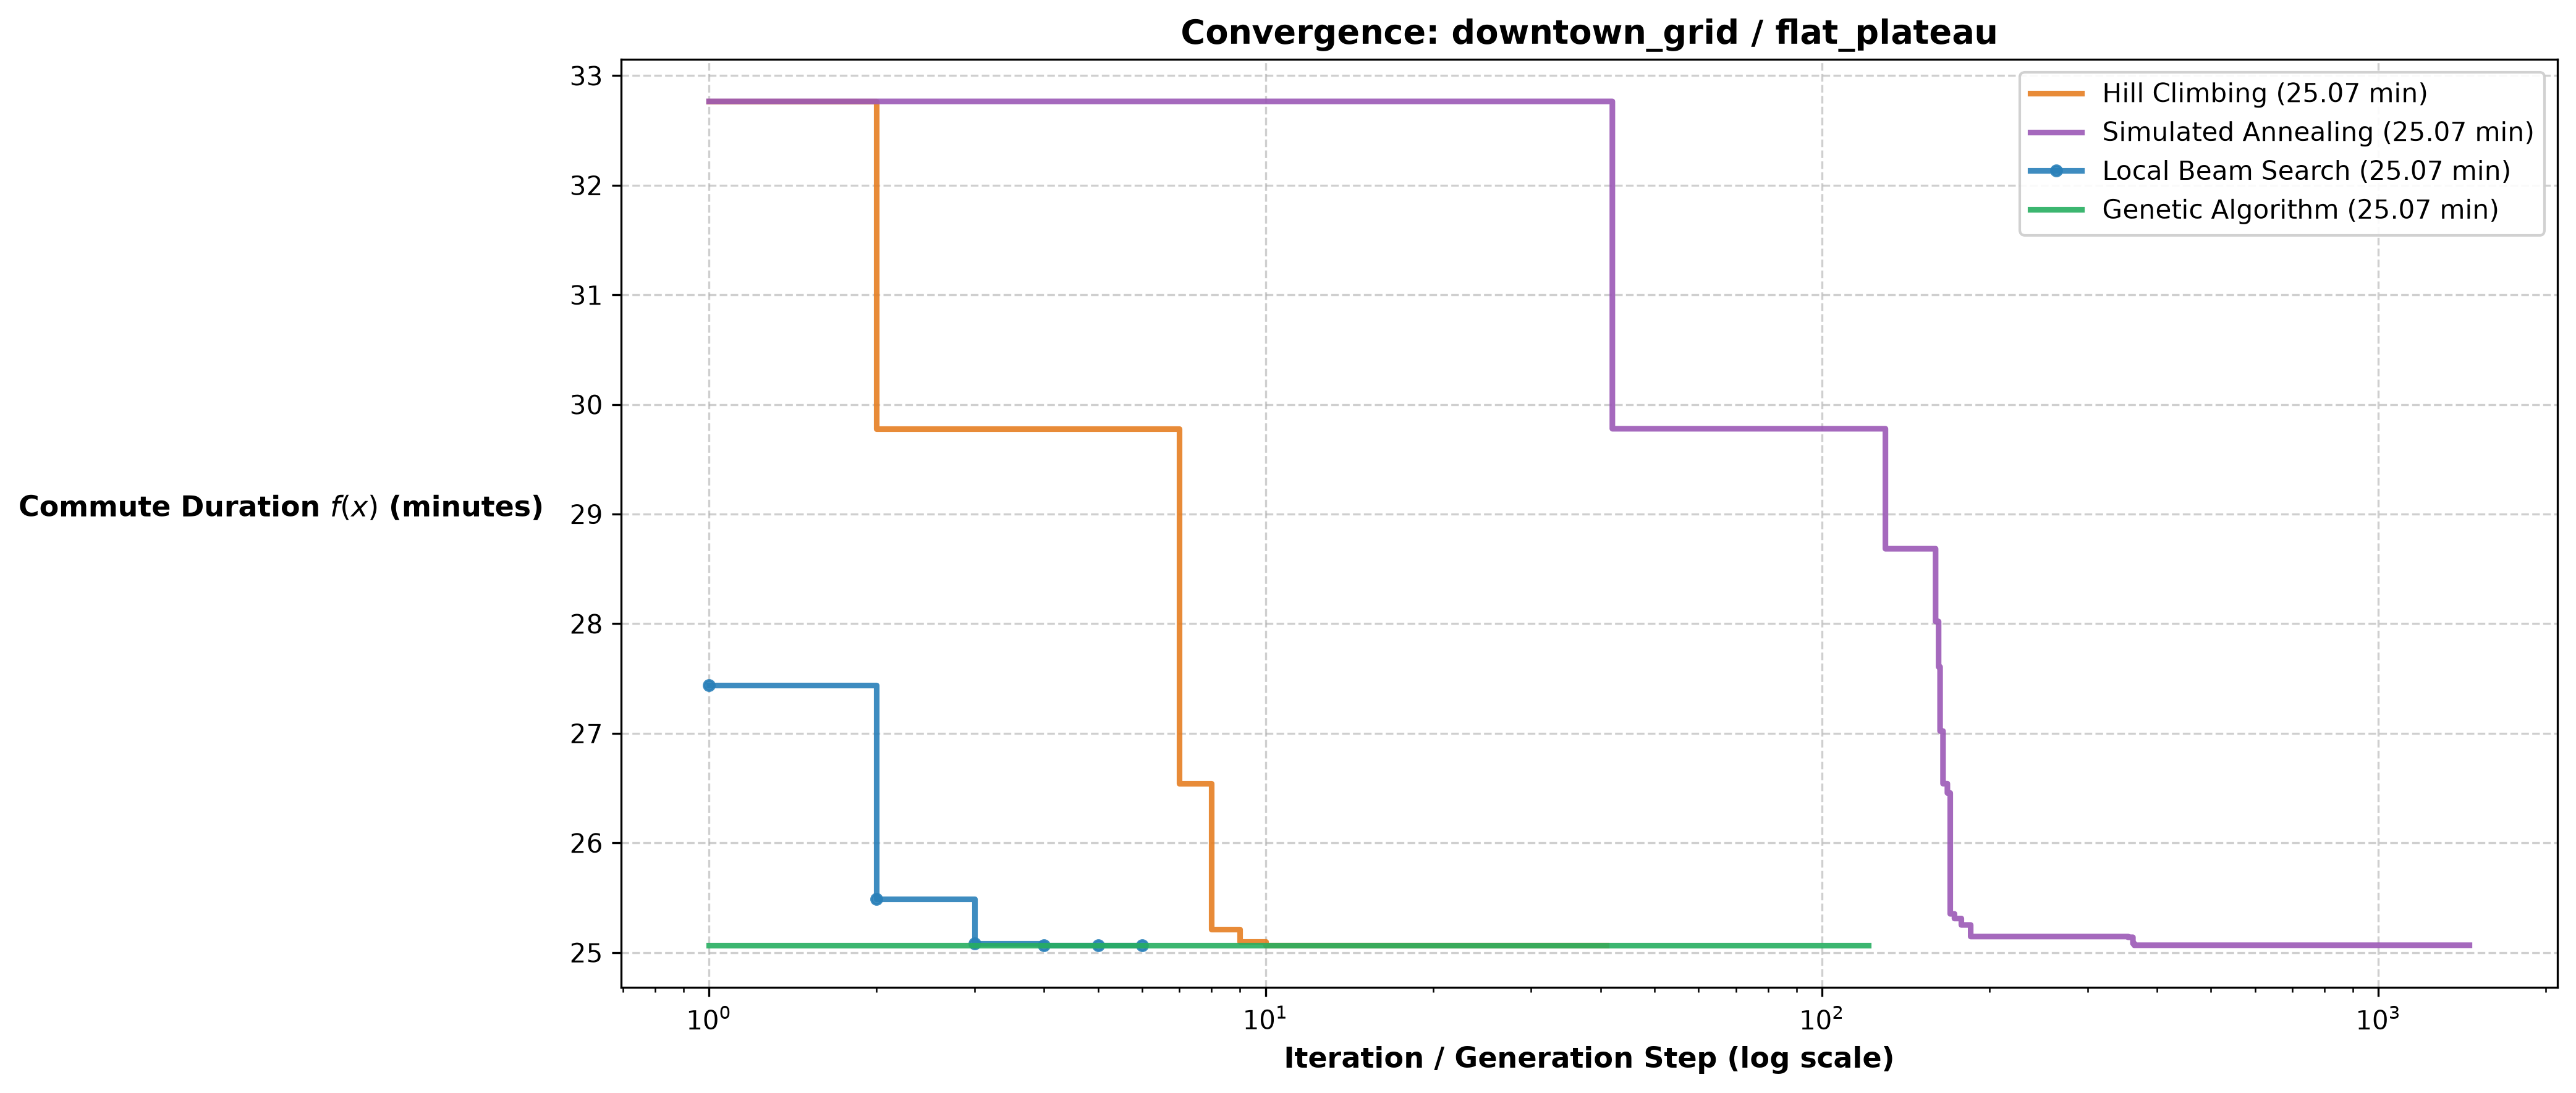
\includegraphics[width=0.49\textwidth]{figures/flat_plateau.png}\hfill
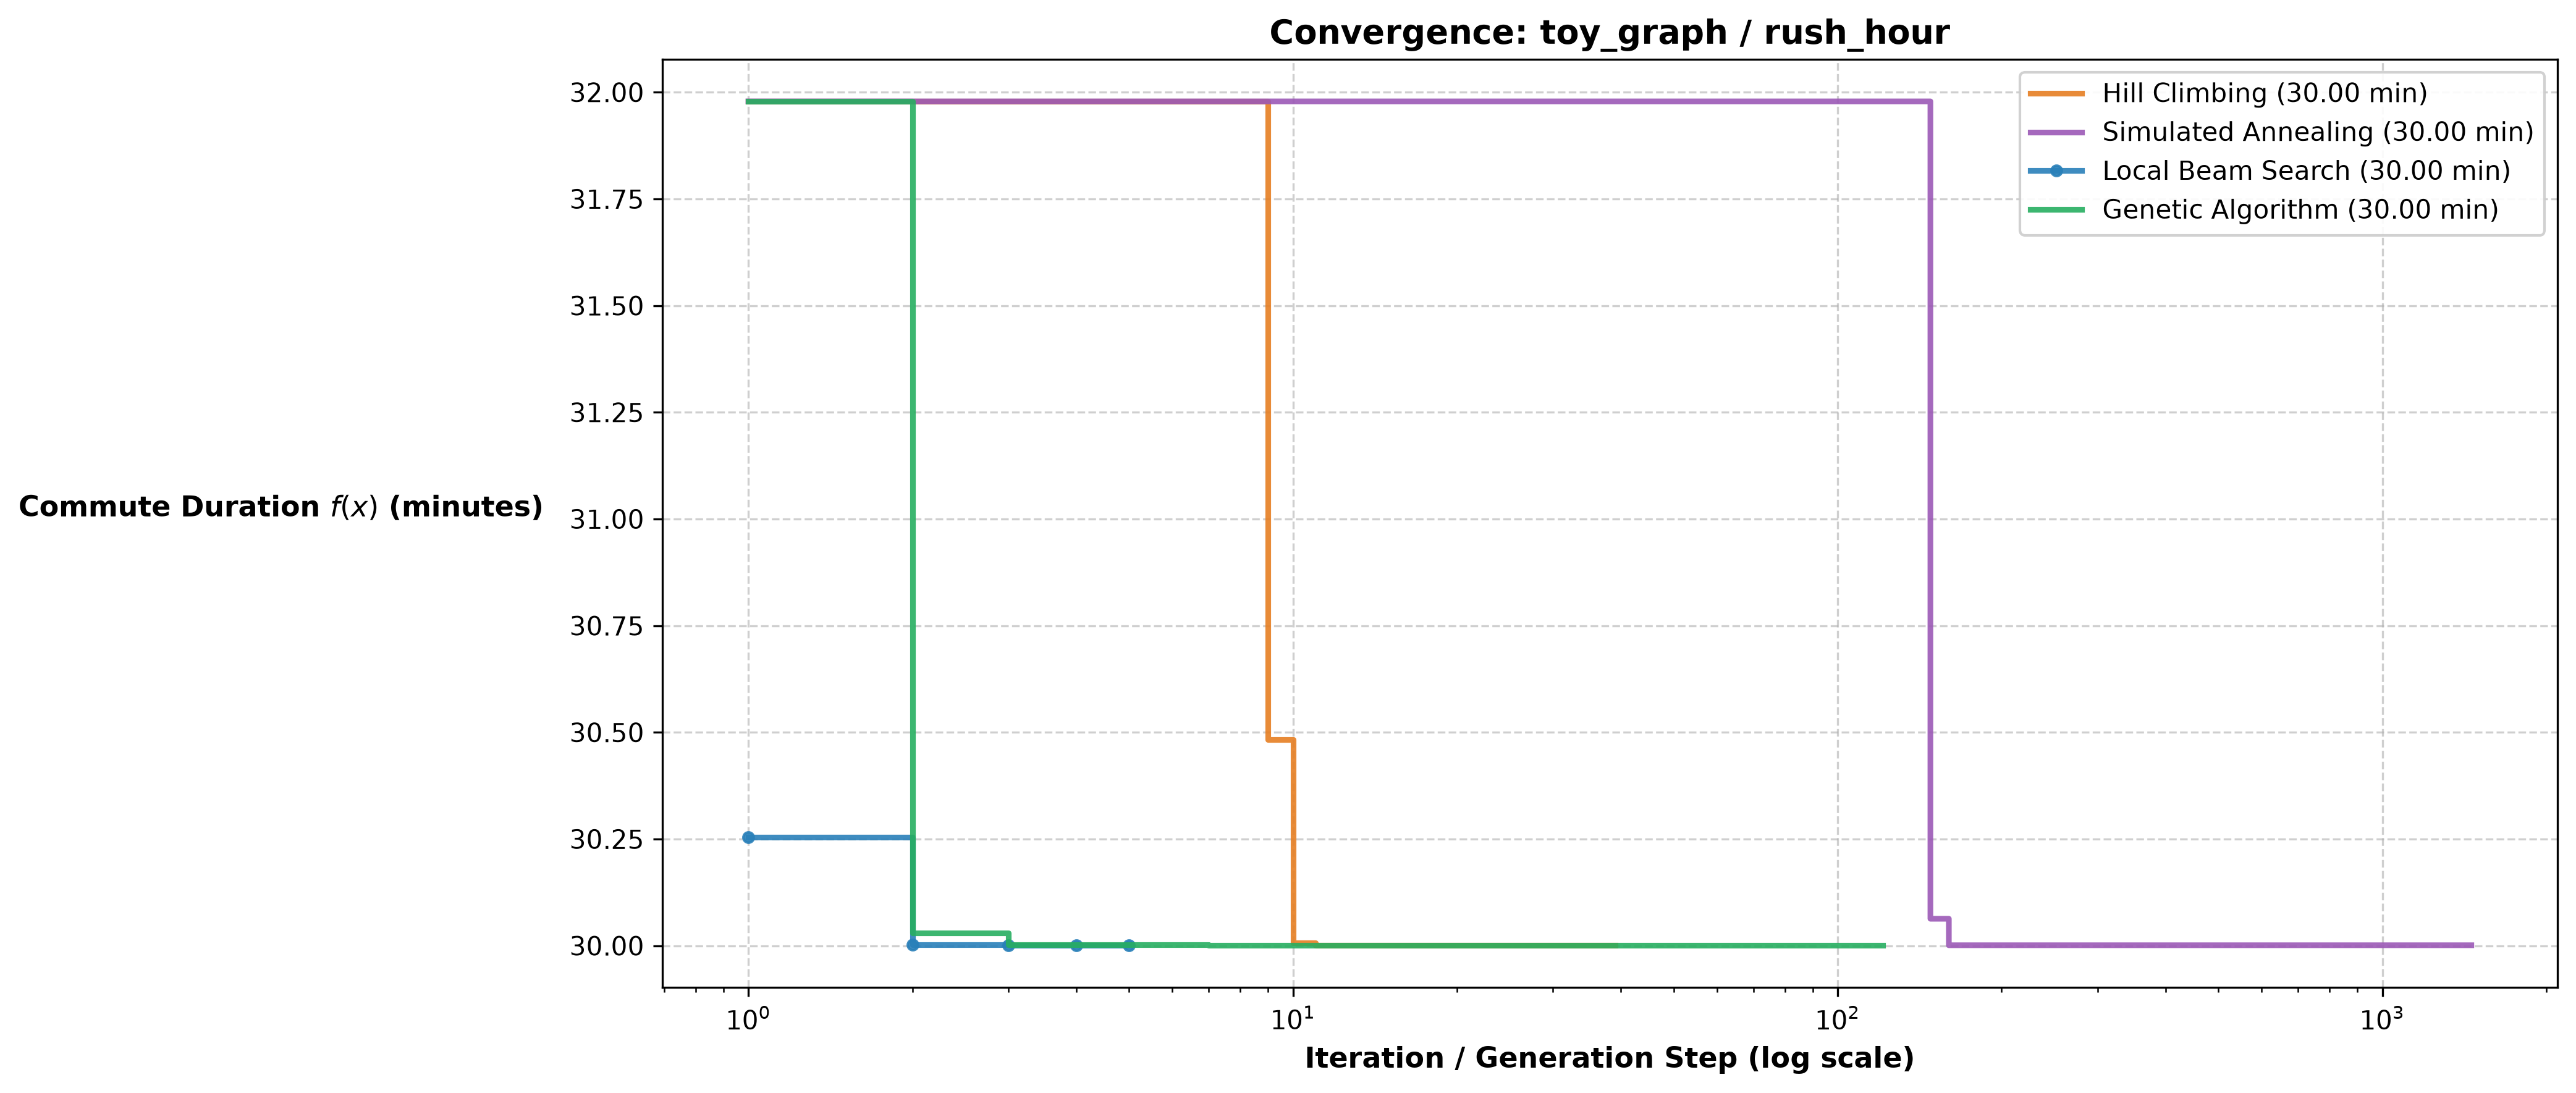
\includegraphics[width=0.49\textwidth]{figures/rush_hour.png}\\[4pt]
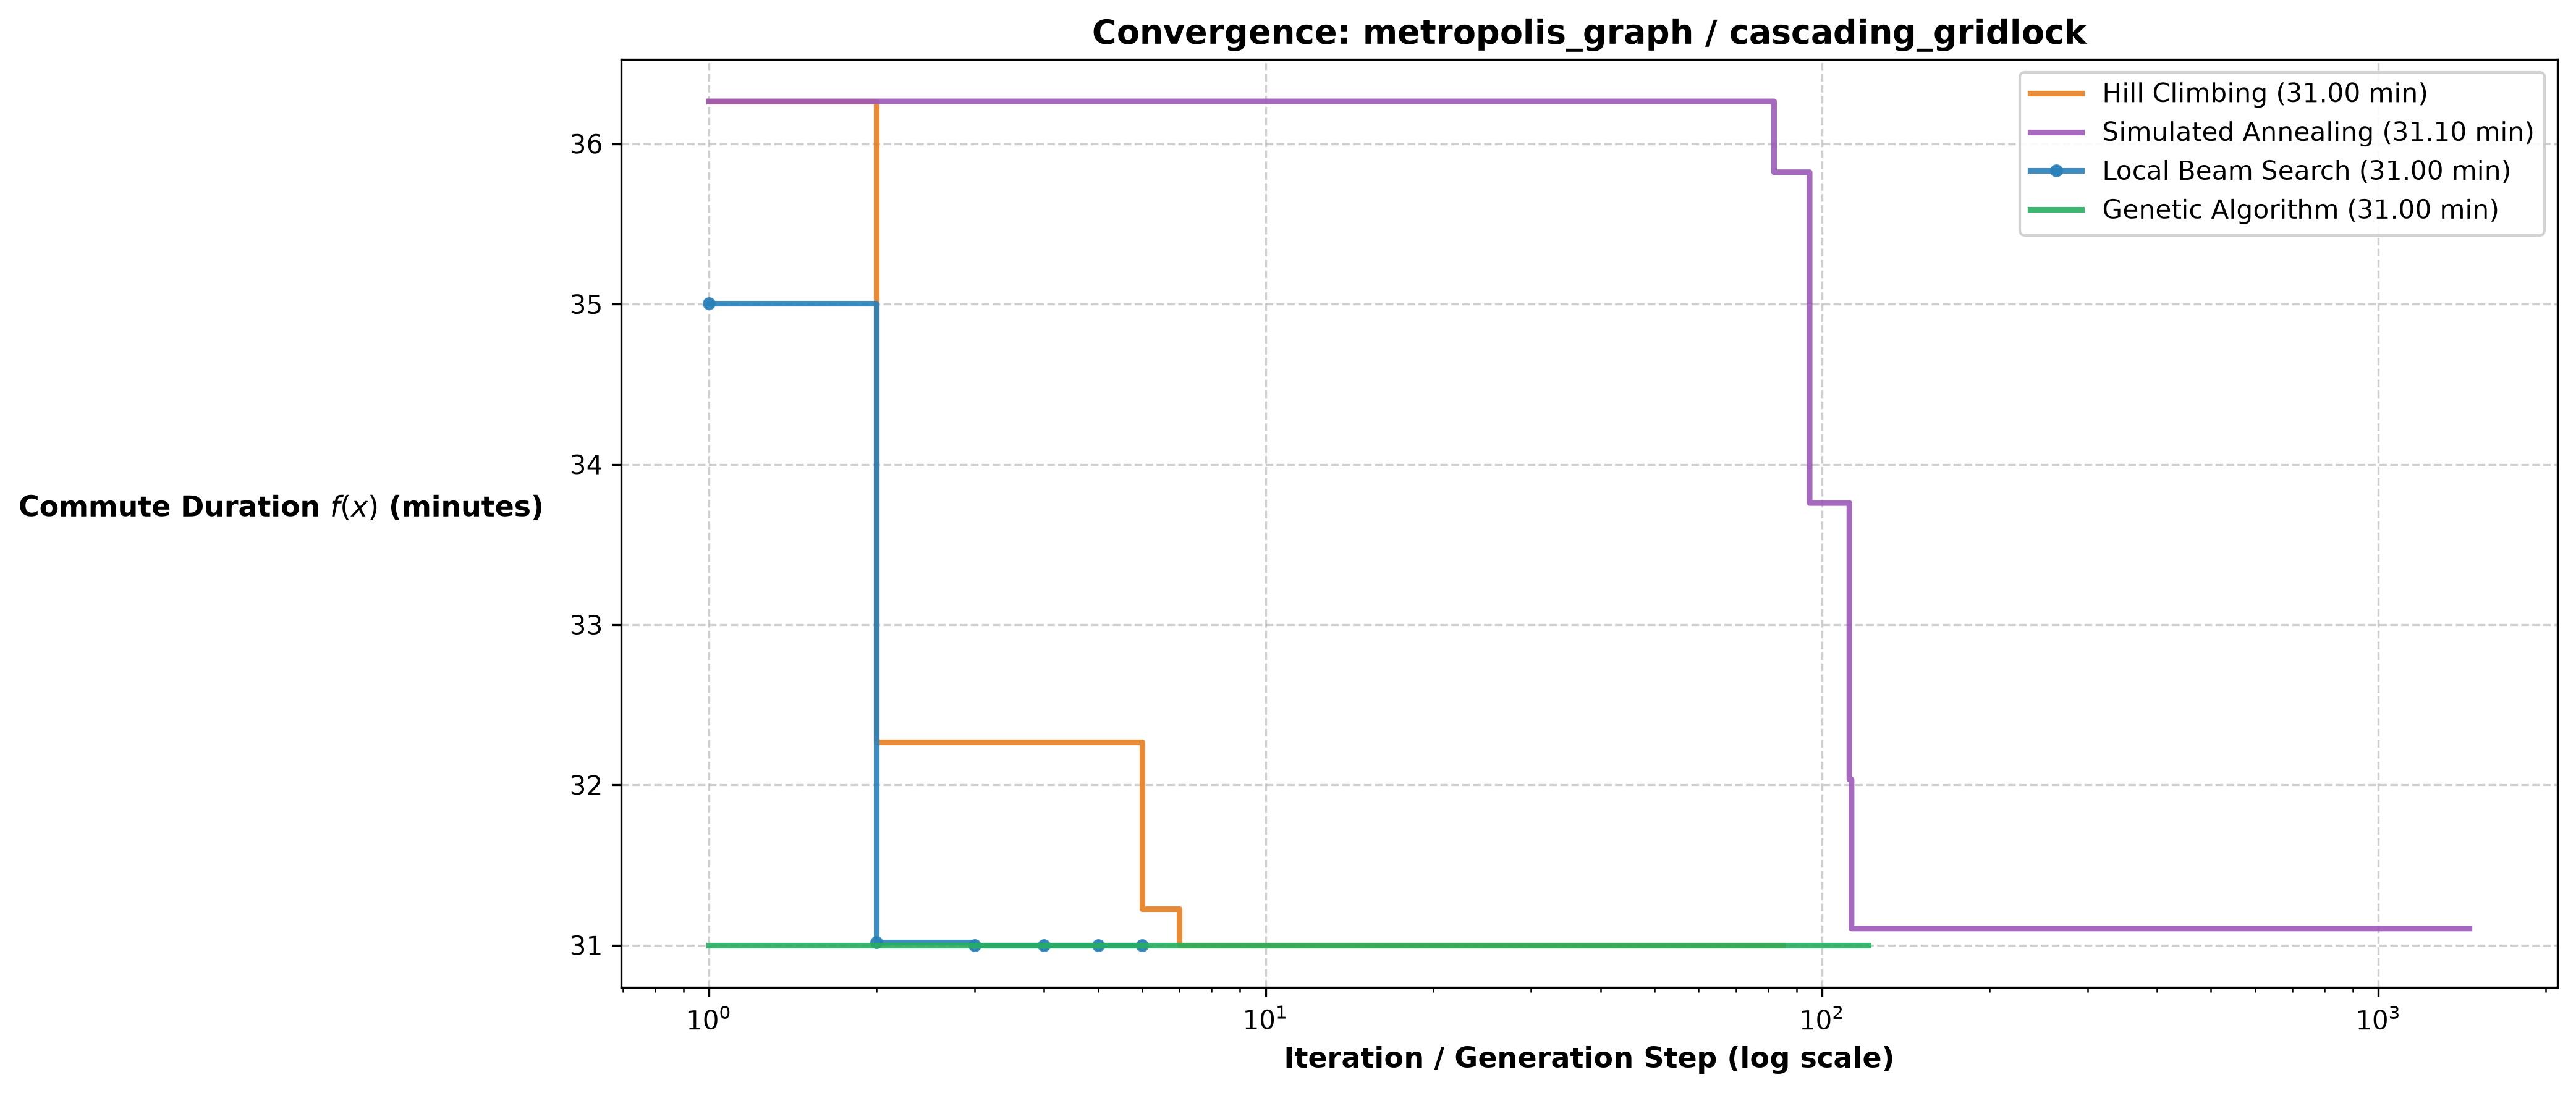
\includegraphics[width=0.49\textwidth]{figures/cascading_gridlock.png}\hfill
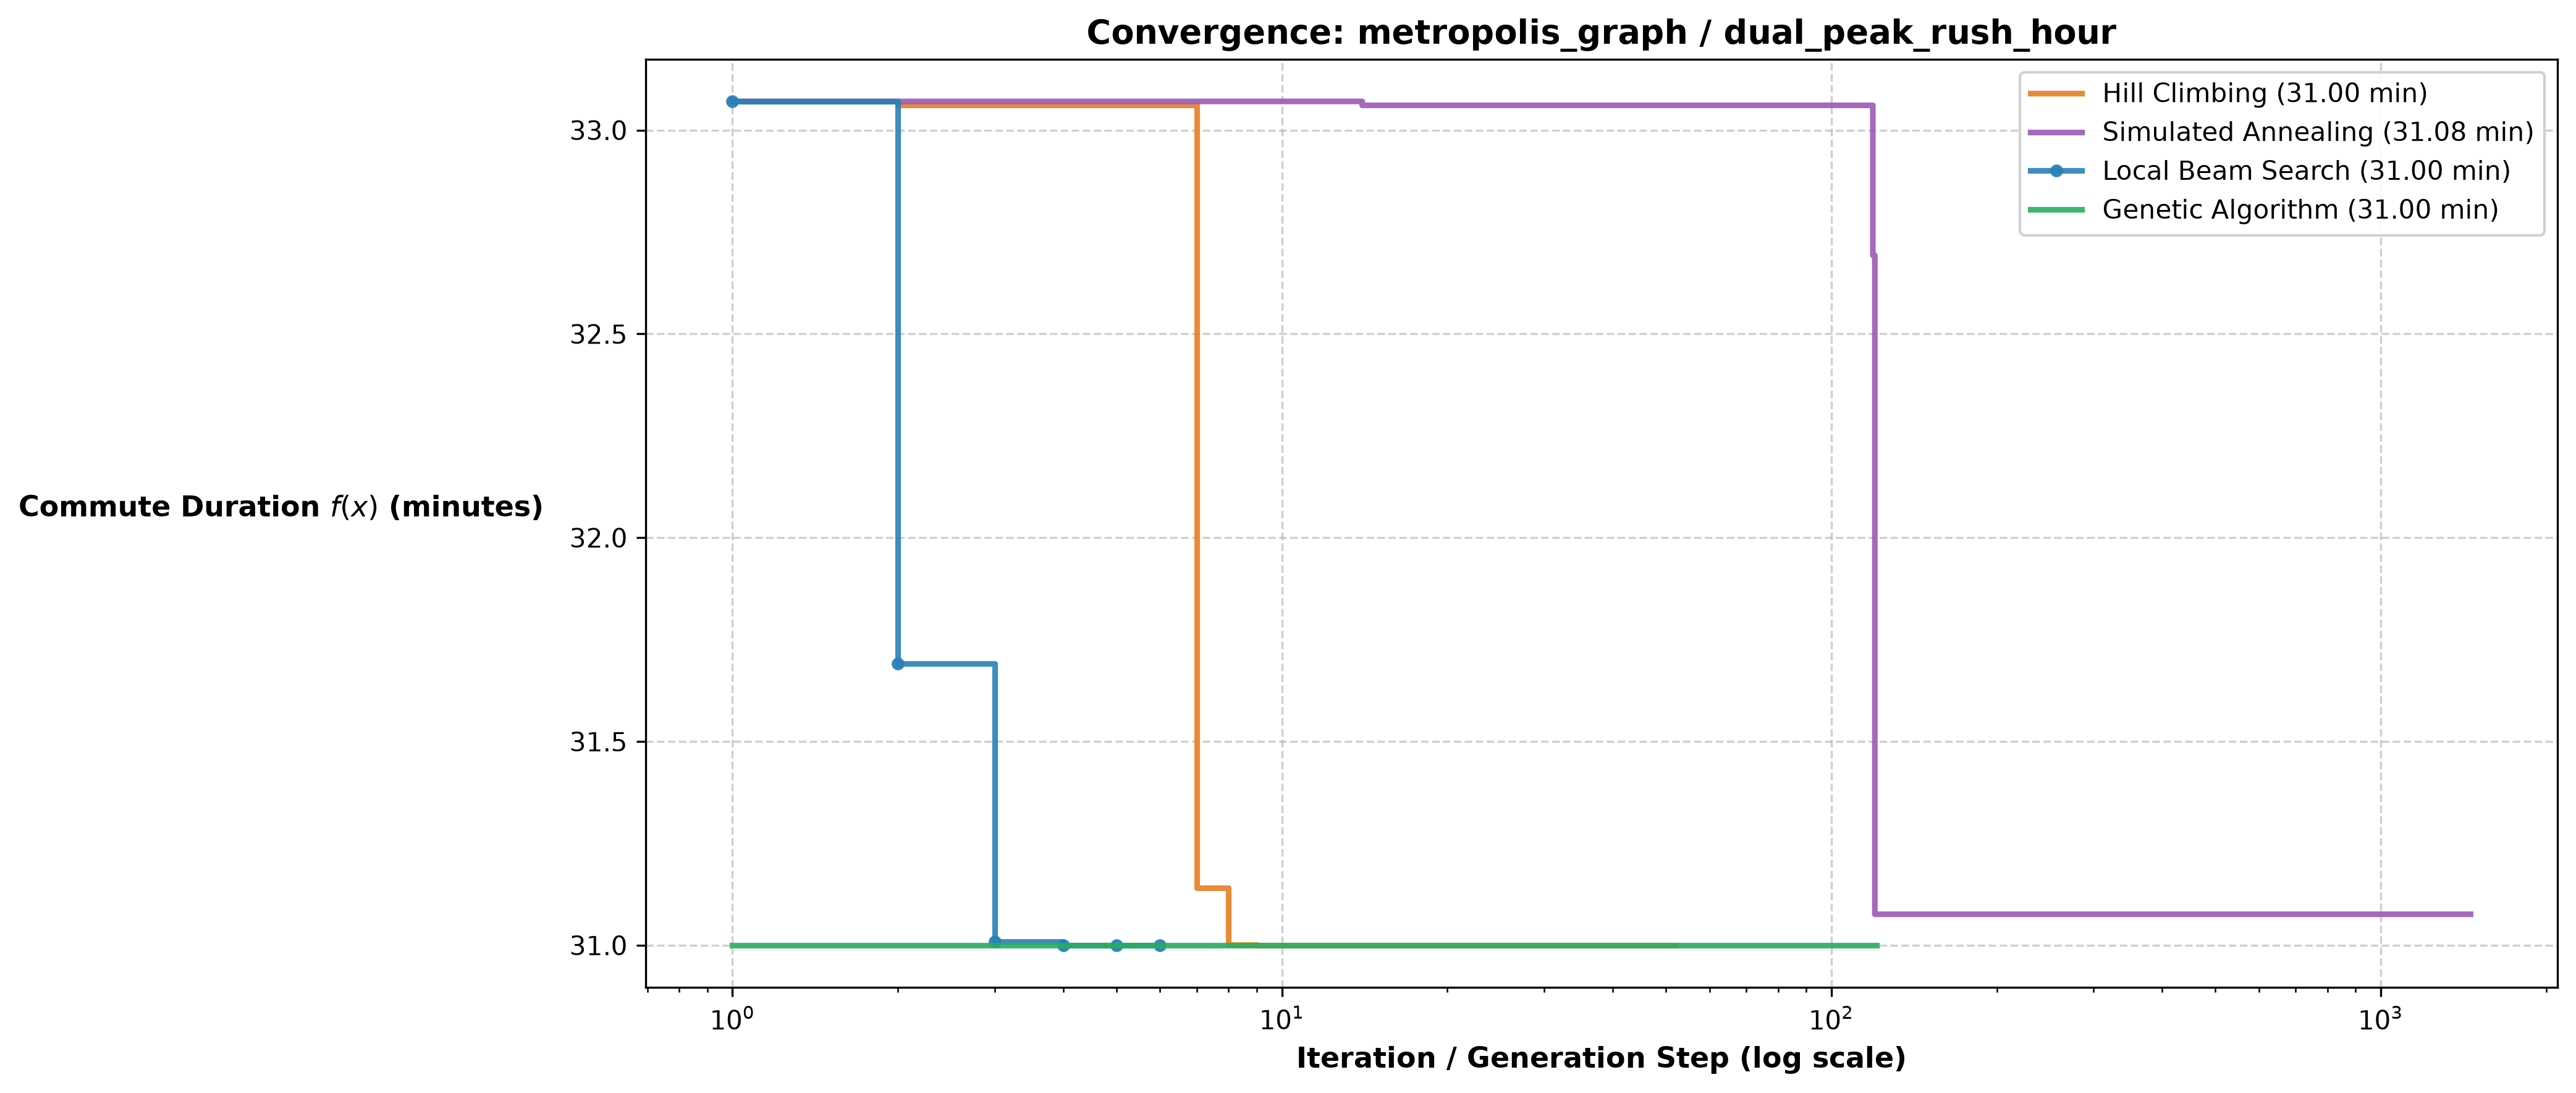
\includegraphics[width=0.49\textwidth]{figures/dual_peak_rush_hour.png}\\[4pt]
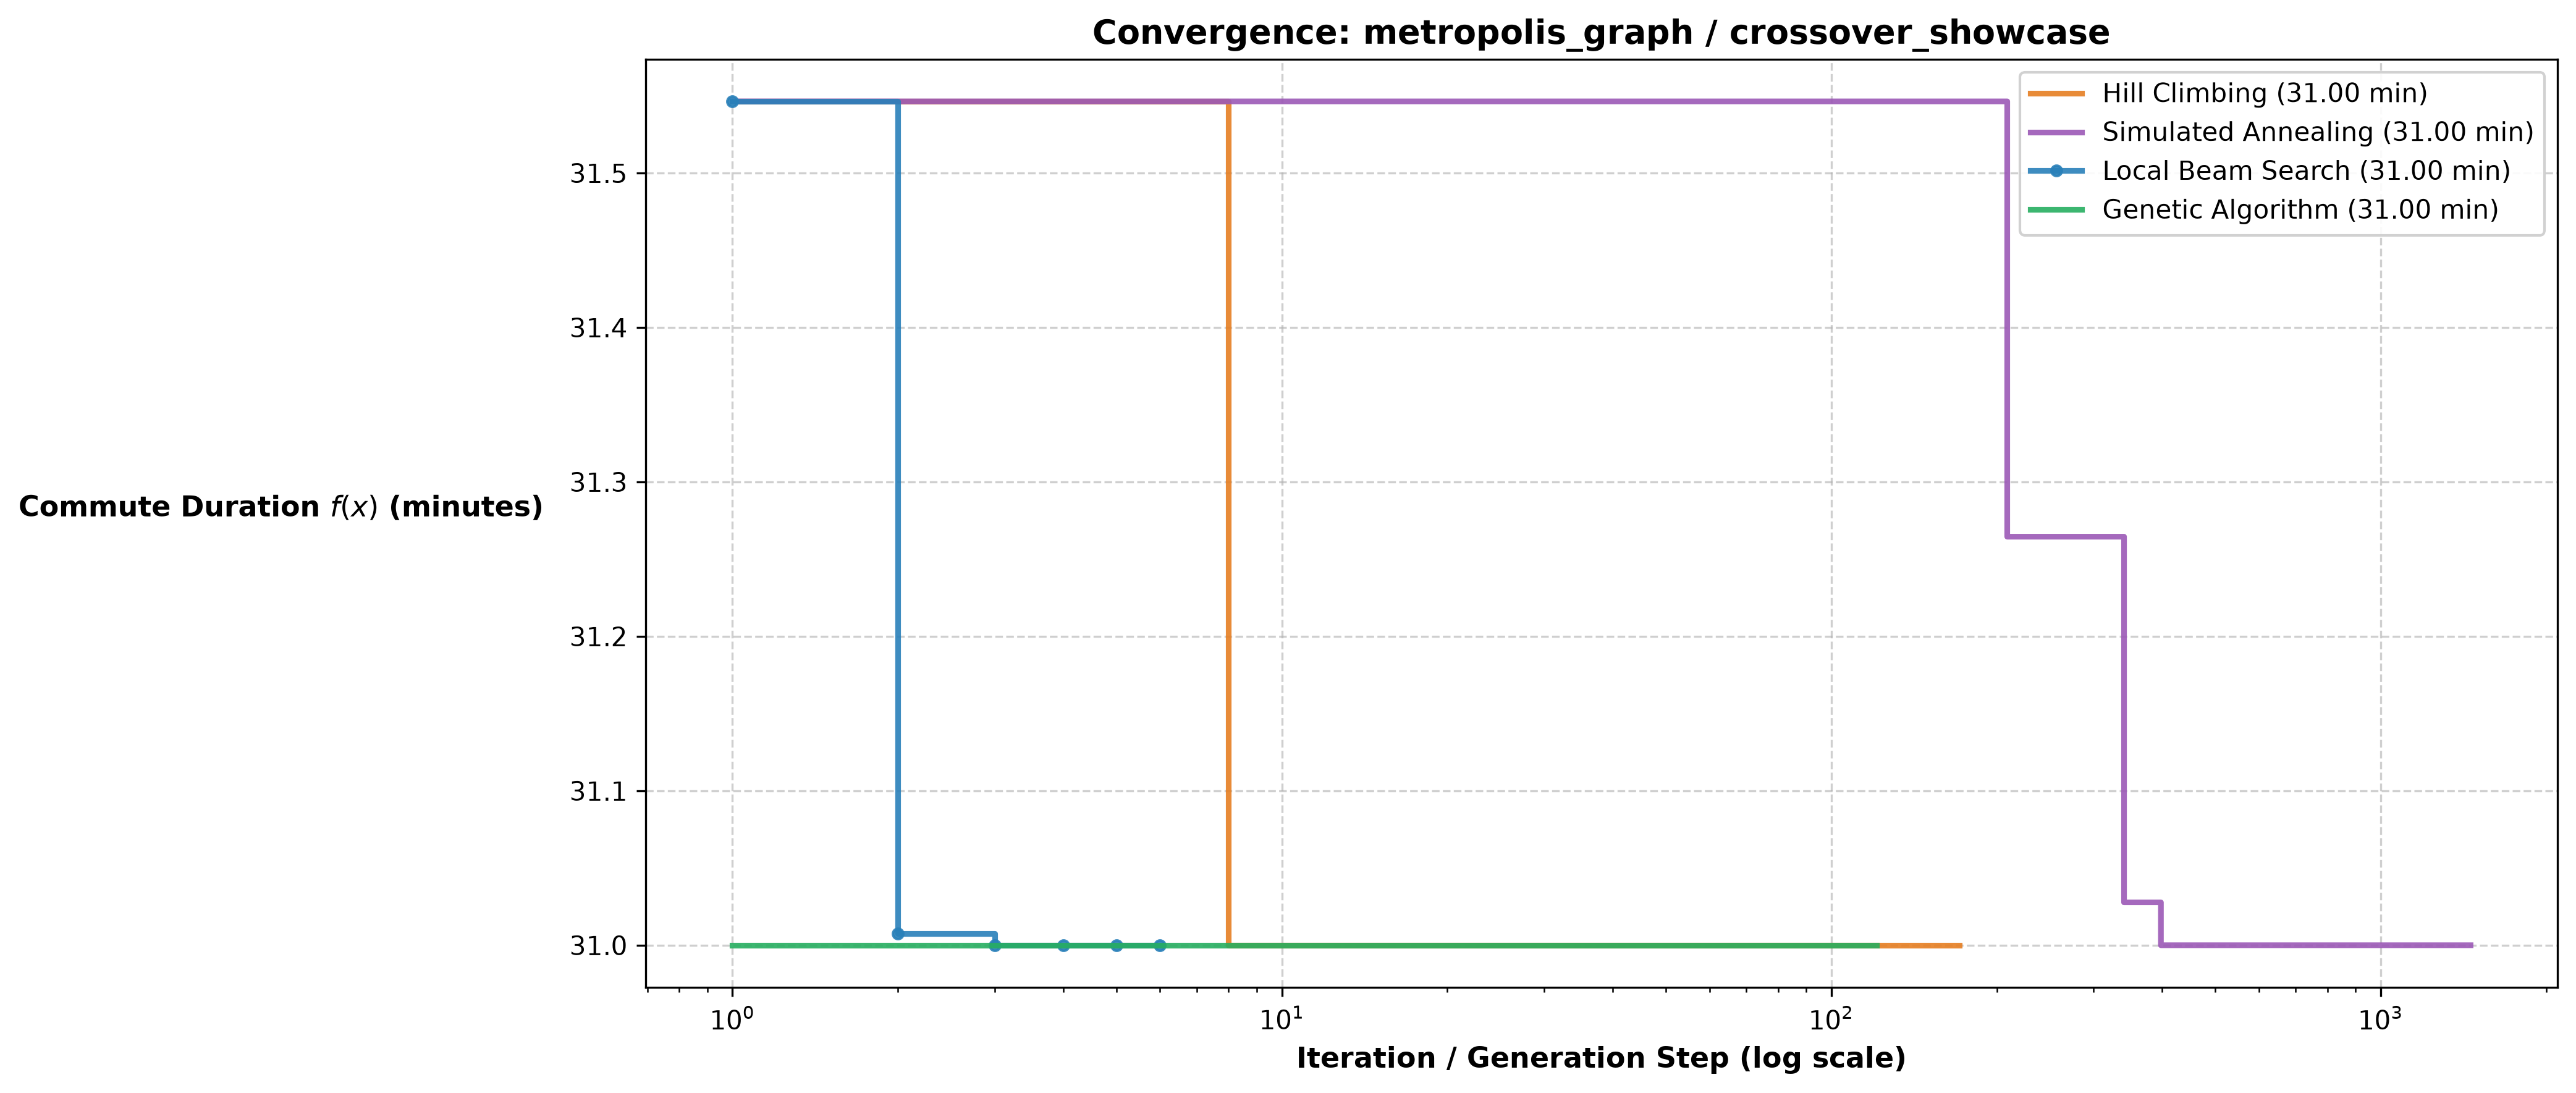
\includegraphics[width=0.49\textwidth]{figures/crossover_showcase.png}
\caption{Convergence on the small-map scenarios.}
\label{fig:others}
\end{figure}

% =====================================================================
\section{Analytical Questions}

\subsection*{Question 1: Continuous optimization and gradient descent}
\addcontentsline{toc}{subsection}{Question 1: Gradient descent}

\textbf{Path.} Gradient descent needs a continuous variable and a gradient. A path is a discrete
sequence of nodes: there is no ``small step'' from one path to another, $x - \alpha\nabla f(x)$
has no meaning for it, and an intermediate value between two routes is not a route. Most nearby
values would not be connected paths anyway.

\textbf{Departure time.} For a fixed $P$ this is possible, if we treat $t$ as continuous. With
$a_0 = t$ and $a_{i+1} = a_i + t^{\text{base}}_i (1 + C_i(a_i))$, the objective is
$f(t) = a_m(t) - t$, and the chain rule gives
\[
f'(t) = \prod_{i=0}^{m-1} \left( 1 + t^{\text{base}}_i \, C_i'(a_i) \right) - 1 .
\]
The conditions on $C_e(t)$ are:
\begin{itemize}
  \item \textbf{Differentiable}, with a Lipschitz-continuous derivative so a safe step size
  $\alpha$ exists. A sum of Gaussians satisfies this.
  \item \textbf{FIFO}: $1 + t^{\text{base}}_e C_e'(t) \ge 0$, so leaving later never means arriving
  earlier. For one Gaussian the steepest slope is about $0.61\,A/\sigma$, so we need
  $0.61\, t^{\text{base}} A / \sigma \le 1$. A short and heavy peak can break this: base 6.6,
  $A = 7$ and $\sigma = 20$ gives 1.4.
\end{itemize}
Even then $f$ is not convex when there are several peaks, so gradient descent only finds a local
minimum. The result must also be clipped to $[t_{\min}, t_{\max}]$ and snapped back to the grid.

\subsection*{Question 2: Local search vs.\ incremental search}
\addcontentsline{toc}{subsection}{Question 2: Local vs.\ incremental search}

\textbf{Why a complete configuration?} The cost of an edge depends on the arrival time, which depends
on the departure time and on all earlier edges. So $P$ and $t_{\text{start}}$ are coupled, and the
natural question is about the whole trip. A complete state can always be evaluated, it is always a
usable answer if we stop early, and memory use is small.

\textbf{When is time-dependent Dijkstra in trouble?}
\begin{itemize}
  \item \textbf{Many departure times.} One run answers one departure time. Here it needs 37 runs,
  and more on a finer grid.
  \item \textbf{FIFO violations.} Optimal sub-paths are no longer guaranteed, because arriving later
  at a node can be better. Then Dijkstra's greedy settling is not correct.
  \item \textbf{Whole-route constraints or objectives}, such as limits on turns or tolls, or costs
  that do not add up edge by edge. The state must grow to include them.
  \item \textbf{Very large networks} with changing traffic and limited time. Local search still gives
  an answer at any moment, though without an optimality guarantee.
\end{itemize}
With FIFO and a small set of departure times, Dijkstra is actually exact and a very good option.

\subsection*{Question 3: Local Beam Search vs.\ Genetic Algorithm}
\addcontentsline{toc}{subsection}{Question 3: Beam Search vs.\ GA}

\textbf{Advantage of crossover.} Beam can only reach a neighbor of a state it already holds, which
means a change of up to 4 edges at a time, and it keeps only the top $K$. Crossover can join the good
start of one route with the good end of another in one step, and the child can be far from both
parents. Tournament selection also lets weaker individuals survive, and their sections may turn out to
be useful later. On \col{big\_city} GA reached 55.43 against 73.82 for Beam, although GA's bigger
population and random start also helped.

\textbf{Population collapse.} The strict form is blocked: taking the best state per distinct path
stops the beam from becoming one route at 8 adjacent times. A softer collapse still seems to happen,
because 8 distinct paths can all be small detours of a single route. Beam stopping after 8 steps at
73.82 on \col{big\_city} fits that picture. Ways to keep diversity:
\begin{itemize}
  \item limit how many beam slots can come from one parent (stochastic beam search also helps);
  \item require a minimum edge difference between the paths in the beam;
  \item replace the worst slots with fresh random states when the beam stalls.
\end{itemize}

\subsection*{Question 4: Plateaus and sideways moves}
\addcontentsline{toc}{subsection}{Question 4: Plateaus and sideways moves}

\textbf{Real scenarios.}
\begin{itemize}
  \item \textbf{Symmetric streets.} In \col{downtown\_grid} all blocks take 5 minutes, and in
  \col{flat\_plateau} they have the same congestion. Home, G1, G5 and Home, G4, G5 therefore cost
  exactly the same.
  \item \textbf{Off-peak departures.} Far from every peak the Gaussian tail is almost zero. On the
  path above, leaving at 09:55 instead of 10:00 changes the trip by only about 0.03 minutes
  (near-flat, a shoulder).
\end{itemize}
Note that my code treats a move as sideways only if the costs match within $10^{-9}$. So symmetric
routes count as plateaus, while the shoulder case counts as a tiny improvement.

\textbf{Effect of \col{max\_sideways}.} Each sideways step costs a full neighborhood scan, so the worst
case adds $(\text{restarts} + 1) \times \text{max\_sideways}$ scans. With a value of 0, the climb ends at the
first exact tie. In my runs the limit of 100 was not the bottleneck: the HC run on \col{megacity} took
about 127 steps across all 11 climbs. A large value is therefore cheap here, and restarts have
more effect on quality. The \col{tabu} set matters as well, because it prevents the budget from being
wasted on moving back and forth.

\subsection*{Question 5: Cooling schedule dynamics}
\addcontentsline{toc}{subsection}{Question 5: Cooling schedule}

\textbf{Initial temperature.} If $T_0$ is too high, SA behaves like a random walk and wastes
iterations: at $T = 120$ a move that is 10 minutes worse is accepted with probability $0.92$. My
$T_0 = 120$ is on the high side, since nothing improved on \col{megacity} until $T \approx 9$ (step 320),
and in the seed 42 run SA never beat its starting state at all.
If $T_0$ is too low, SA becomes hill climbing from the first step and stays in the starting valley.

\textbf{Cooling rate.} With $T_0 = 120$ and $T_{\min} = 0.001$, the rate decides the number of steps:

\begin{table}[H]
\centering
\begin{tabular}{lll}
\toprule
$\alpha$ & \textbf{Iterations} & \textbf{Expected behavior} \\
\midrule
0.5   & 17 & Quenching: a few random moves, then frozen near the start. \\
0.992 (mine) & 1457 & Random walk first, then a real descent, then frozen. \\
0.999 & 3000 (limit) & Ends at $T \approx 6$, so it is still accepting many worse moves. \\
\bottomrule
\end{tabular}
\end{table}

\noindent The last row is easy to miss: $\alpha = 0.999$ needs about 11700 iterations to cool fully,
so \col{max\_iterations} has to be raised with it. These values follow from the formula. A slower
schedule gives better quality in theory, but costs more runtime, because each SA iteration also builds
a whole neighborhood.

\subsection*{Question 6: Crossover disjointness and epistasis}
\addcontentsline{toc}{subsection}{Question 6: Crossover and epistasis}

\textbf{Disjoint parents.} The origin and destination are skipped when looking for pivots, so the
candidate list stays empty. The fallback then takes one parent at random with the blended time and
returns a random neighbor from \col{get\_neighbors}, which only produces valid states. If there are no
neighbors, it returns that parent with the blended time, which is still valid. So a broken child
cannot come out. The same fallback is used if a splice would repeat a node, since those are filtered
out first.

\textbf{Why can good parents give a bad child?} The value of an edge depends on when we reach it, so
genes strongly interact:
\begin{itemize}
  \item \textbf{Timing of the tail.} A tail that was good in parent 2 was good at parent 2's arrival
  time. With a different head, the child reaches it later or earlier and may hit a wave.
  \item \textbf{Blended time.} One parent may leave before the peak and the other after it. Both are
  good, but a time between them can land right on the peak.
  \item \textbf{Trap edges.} A parent may use a highway only because it reaches it before the
  congestion. The child can inherit the highway without the timing.
\end{itemize}

\subsection*{Question 7: Combinatorial state space}
\addcontentsline{toc}{subsection}{Question 7: State space size}

\textbf{Bound.} With $b$ choices at each of $L$ steps, the number of paths of about that length is
close to $b^L$, so
\[
|\mathcal{X}| \;\lesssim\; N_t \cdot b^{L} .
\]
A strict bound that holds for any graph counts ordered choices of the intermediate nodes, using
simple paths only:
\[
|\mathcal{X}| \;\le\; N_t \sum_{k=0}^{|V|-2} \frac{(|V|-2)!}{(|V|-2-k)!} \;\le\; N_t \cdot e \cdot (|V|-2)! .
\]

\textbf{Why not brute force?} The growth is exponential in $L$. My \col{megacity} map is small
($|V| = 168$, $b = 393/168 \approx 2.34$, $L = 24$ hops across the grid without express links, $N_t = 37$), and it still
gives about $2.7 \times 10^{10}$ states for that length alone. At an optimistic $10\,\mu$s per evaluation
this takes about 3 days, and longer paths make it far worse. A real city with $b \approx 2.5$ and
$L \approx 100$ has around $10^{40}$ paths, which no hardware can enumerate. Local search only looks at
a tiny part of this space and needs little memory, at the cost of having no optimality guarantee.

\end{document}
